\section{Selective mixture gradients and control variates}
\label{sec:hybrid}

The model-score recursion and the choice of mixture-gradient estimator are
separate decisions. Fisher's identity does not require differentiation of
every resampling draw. Mixture expectation derivatives may nevertheless be
needed for proposal learning, sensitivity calculations, or a separately
defined finite program. In those settings, using IWSG for every continuous
movement can introduce avoidable variance.

Consider a single component $Z=\mu+h\varepsilon$, with
$\varepsilon\sim\mathcal N(0,1)$ and fixed $h>0$. For the affine function
$\phi(z)=az+b$, the exact derivative of $\mathbb E\phi(Z)$ with respect to
$\mu$ is $a$. The location-score estimator and the pathwise estimator are
\begin{equation}
 G_{\rm IW}=(a\mu+b+ah\varepsilon)\frac{\varepsilon}{h},
 \qquad G_{\rm PW}=a.
 \label{eq:gaussian-gradient-estimators}
\end{equation}
Both have mean $a$. Using
$\mathbb E\varepsilon^2=1$, $\mathbb E\varepsilon^3=0$, and
$\mathbb E\varepsilon^4=3$ gives
\begin{equation}
 \operatorname{Var}(G_{\rm IW})
   =\frac{(a\mu+b)^2}{h^2}+2a^2,
 \qquad \operatorname{Var}(G_{\rm PW})=0.
 \label{eq:gaussian-gradient-variance}
\end{equation}
The constant part of the integrand, which has zero true derivative, is
responsible for the diverging term. Subtracting the detached baseline
$\phi(\mu)$ from the score-function term produces $a\varepsilon^2$, whose
variance is $2a^2$. No bias was removed; a needless source of variance was
removed. Figure~\ref{fig:gradient-variance} makes the bandwidth effect explicit.

\begin{figure}[tbp]
\centering
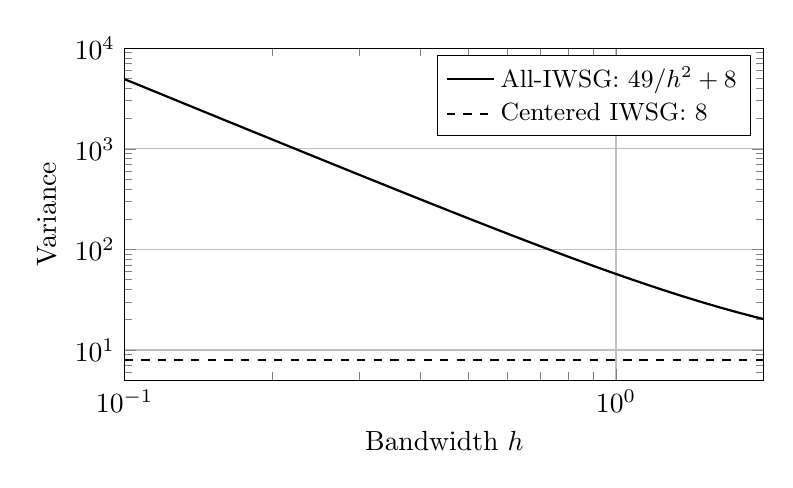
\begin{tikzpicture}
\begin{loglogaxis}[
 width=.80\textwidth,height=5.8cm,
 xlabel={Bandwidth $h$},ylabel={Variance},
 xmin=.1,xmax=2,ymin=5,ymax=10000,
 grid=major,legend style={at={(.98,.98)},anchor=north east,font=\small},
 legend cell align=left]
 \addplot[black,thick,domain=.1:2,samples=80]{49/(x*x)+8};
 \addlegendentry{All-IWSG: $49/h^2+8$}
 \addplot[black,dashed,thick,domain=.1:2]{8};
 \addlegendentry{Centered IWSG: $8$}
\end{loglogaxis}
\end{tikzpicture}
\caption{A narrow component can make an unbiased importance-weight derivative
noisy. For $a=2$, $\mu=3$, and $b=1$, the uncentered variance grows as
$49/h^2+8$, while the centered variance stays at 8. The pathwise derivative
has zero variance and therefore does not appear on the logarithmic axis.
These curves are the exact calculation in
\eqref{eq:gaussian-gradient-variance}, not filtering benchmark results.}
\label{fig:gradient-variance}
\end{figure}

This example isolates one smooth component. Younis's argument concerns an
additional difficulty: implicit mixture reparameterizations may move samples
between widely separated modes and have large variance. The example does
not refute that finding. It motivates treating continuous motion within a
component differently from a change in component probability.

\begin{samepage}
Let $m_\theta(z)=\sum_iw_i(\theta)k_{i,\theta}(z)$, sample
$I\sim\operatorname{Cat}(w)$, and represent a component sample by
$Z=T_{I,\theta}(\varepsilon)$ with parameter-independent base noise.
Assume positive component weights and sufficient regularity and integrability
to differentiate each component expectation. Differentiating their sum gives
\begin{align}
 J(\theta)&=\sum_iw_i\,
             \mathbb E_\varepsilon[\phi_\theta(T_{i,\theta}(\varepsilon))],
 \notag\\
 \nabla_\theta J
 &=\sum_i(\nabla_\theta w_i)\,
             \mathbb E_\varepsilon[\phi_\theta(T_{i,\theta}(\varepsilon))]
   +\sum_iw_i\,
             \mathbb E_\varepsilon\!\left[
                 \frac{d}{d\theta}\phi_\theta(T_{i,\theta}(\varepsilon))
             \right].
 \label{eq:hybrid-component-derivation}
\end{align}
\end{samepage}
For a baseline $c$ independent of the current component and noise, a resulting
estimator is
\begin{equation}
 G_{\rm hybrid}
 =\frac{d}{d\theta}\phi_\theta(T_{I,\theta}(\varepsilon))
  +(\phi_\theta(Z)-c)\nabla_\theta\log w_I.
 \label{eq:hybrid-estimator}
\end{equation}
The first term holds $I$ fixed and includes both the explicit derivative of
$\phi$ and movement of $T_{I,\theta}$. The second accounts for changing
component probabilities. Its baseline has zero expectation because
$\sum_iw_i\nabla\log w_i=\nabla\sum_iw_i=0$. A component-dependent baseline
does not have this cancellation unless its compensating term is retained.
The baseline may depend on $\theta$ or past information, but it is held fixed
within this gradient-estimation operation.

The categorical term can be averaged over its conditional component
responsibilities, or components can be enumerated and sampled with a
stratified allocation. Such changes have different costs and covariances with
the pathwise term. Reducing the variance of one term does not automatically
rank the complete estimator. A baseline fitted from the same sample also
requires a justified leave-one-out or independent-fit construction; otherwise
the claimed zero-mean property can fail.

The official Younis code contains an
\texttt{ImportanceImplicitHybrid} branch that separates derivatives of
component locations/bandwidths from derivatives of weights
\citep{youniscode2023}. Its continuous part uses implicit mixture
reparameterization. Equation~\eqref{eq:hybrid-estimator} instead uses a
componentwise pathwise derivative and is a distinct proposal. Neither the
presence of that branch nor the single-Gaussian calculation establishes
benefit for the full BayesFilter recursion.

Finally, the identity being estimated must remain explicit. A hybrid may
estimate the same mixture expectation derivative as IWSG while differing
sample by sample. Substituting it into a fixed-anchor finite program and
claiming the same derivative would require a new argument. The finite
program, the expected stochastic objective, and the underlying model score
cannot share a name merely because their estimators agree in a small example.

\subsection{What a control variate can accomplish}

For a baseline score estimate $G$ and a control $C$ with known mean $c$, define
\begin{equation}
 G_{\rm cv}=G-\beta(C-c),\qquad
 \mathbb E G_{\rm cv}=\mathbb E G.
 \label{eq:score-control-variate}
\end{equation}
The equality requires fixed $\beta$, or suitable independence from the
current estimating sample. A vector control may use a coefficient matrix.
A useful correlation can reduce variance and hence MSE, but the baseline
bias is retained. An independently estimated $c$ can be used when its
expectation is correct and its additional uncertainty is included. Merely
naming a KDM score as the control does not provide its mean.

The earlier residual decomposition is still an exact algebraic identity:
\begin{equation}
 L_0^N=A_h+\left(L_0^N-A_h\right),\qquad
 \dd L_0^N=\dd A_h+\dd\left(L_0^N-A_h\right).
 \label{eq:residual}
\end{equation}
Dropping the residual changes the target. Computing both terms exactly,
however, gives the original calculation back and supplies no automatic
variance or cost reduction. The useful additional ingredient would be a
cheap, accurately integrable approximation and a residual whose expectation
can be estimated with less error or work.

For example, let $\widetilde p_\theta(x,y)$ be a tractable approximation to
the joint density, with known integral $\widetilde Z(\theta)$. For a proposal
$q$ covering the support of the density difference,
\begin{align}
 Z(\theta)&=\widetilde Z(\theta)
 +\mathbb E_q\!\left[
       \frac{p_\theta(X,y)-\widetilde p_\theta(X,y)}{q(X)}\right],\\
 \nabla_\theta Z(\theta)&=\nabla_\theta\widetilde Z(\theta)
 +\mathbb E_q\!\left[
       \frac{\nabla_\theta p_\theta(X,y)
             -\nabla_\theta\widetilde p_\theta(X,y)}{q(X)}\right].
 \label{eq:joint-surrogate-residual}
\end{align}
The second equality assumes fixed $q$ and valid differentiation under the
integral. If the approximation is close, the residual may be easier to
integrate. The ratio of the resulting estimates still need not be an unbiased
score, and a signed residual estimate can make the likelihood estimate
negative. It is therefore not automatically eligible for pseudo-marginal
inference. The residual formulation deserves a separate comparison if a
tractable approximation can be constructed cheaply; it is not what the
previous integrated KDM experiments implemented.
